\chapter{Single Variable Calculus}

\newpage

\begin{multicols}{2}
\section{Basic}
\subsection{Mängder}
\begin{align*}
  &\quad \text{Naturliga tal: } \mathbb{N} = \{0, 1, 2 , 3 ..  \} \text{ or } \{1, 2 , 3 ..  \} \\
  &\quad \text{Heltal: }\mathbb{Z} = \{.. -2, 1, 0, 1, 2 ..  \} \\
  &\quad \text{Rationella tal: }\mathbb{Q} = \left\{ \frac{a}{b} \Big| \; a,b \in \mathbb{Z} \right\} \\
  &\quad \text{Irrationella tal: }\mathbb{P} = \frac{\mathbb{R}}{\mathbb{Q}}eller \left\{ x | x \in \mathbb{R}, x \notin \mathbb{Q} \right\} \\
  &\quad \text{Reella tal: }\mathbb{R} =  \mathbb{P} \cup \mathbb{Q} \\
\end{align*}

\begin{align*}
  &\quad A \cup B = \{ x:(x \in A) \lor (x \in B)\} \\
  &\quad A \cap B = \{ x:(x \in A) \land (x \in B)\} \\
  &\quad A \setminus B = \{ x:(x \in A) \land (x \notin B)\} \\
  &\quad A^{\text{\#}} = \{ x:(x \in X) \land (x \notin A)\} \\
\end{align*}


\subsection{Intervall}
\begin{align*}
  &\quad \text{Open intervall} = (1,4) \\
  &\quad \text{Closed intervall} = [ \, 1,4 ] \, \\
\end{align*}
\begin{equation}
[ \, a, b ] \, = \{ x | a \leq x \leq b \}
\end{equation}

\begin{equation}
[ \, a, \infty [ \,
\end{equation}
\begin{equation}
] \, -\infty, \infty [ \,
\end{equation}

\textbf{Exempel: Olikheter och intervall}
\begin{equation}
\frac { 2 } { x - 3 } < \frac { 5 } { x }
\end{equation}

\begin{align*}
&\quad \frac{ 2 }{ x - 3 } - \frac{ 5 }{ x } < 0 \\
&\quad \frac{(x) 2 }{x (x - 3)} - \frac{ 5 ( x - 3 )}{ x ( x - 3 ) } < 0 \\
&\quad \frac{ 2 x - 5 x - 15 }{ x ( x - 3 ) } < 0 \\
&\quad \frac{ - 3 x - 15 }{ x ( x - 3 ) } < 0 \\
&\quad \frac{ - 3 ( x - 5 ) }{ x ( x - 3 ) } < 0 \\
&\quad  x \neq 0 , x \neq 3 \\
\end{align*}

Värde tabell:
\begin{center}
\begin{tabular}{ |c|c|c|c|c| } 
 \hline
        & x<0   & 0<x<3 & 3<x<5 & 5<x   \\ 
 x-5    & -     & -     & -     & +     \\ 
 -3     & -     & -     & -     & -     \\  
 x      & -     & +     & +     & +     \\ 
 x-3    & -     & -     & +     & +     \\ 
 hela   & +     & -     & +     & -     \\ 
 \hline
\end{tabular}
\end{center}


\subsection{Funktion}
\begin{itemize}
  \item $f: A \to B$ \\
  \item $A$: domain/definitionsmängd \\
  \item $B$: Målmängd/kodomängd/värdemängd \\
  \item Injektion: alla element $x$ har olika värden $y$
  $f: A \to B, \{{\forall x \in A: x_1 \neq x_2, f(x_1) \neq f(x_2)}\}$
  \item Surjektion: mängd $D$ är definitions mängden
  $\{g: C \to D, g(x)=y, (\forall y \in D \land \exists x \in C)\}$
  \item Bijektion: Injektion $\land$ Surjektion
  \item $f \circ g = f(g(x))$
  \item Begränsad: functionen är inom ett intervall, altså nedåt och uppåt
  \item Begränsat nedåt: functionenn är endast begrensad nedåt
  \item Begränsat uppåt: functionenn är endast begrensad uppåt
  \item Jämn function: altså är den symetrisk, ex: $x^2, \; f(-x)=f(x)$
  \item Udda function: altså är den spefelvänt symetrisk, ex: $x^3, \; f(-x)=-f(x)$
  \item Polynom $p(x)=a_nx^n +a_{n-1}x^{n-1}+ \ldots +a_1x +a_0$
  $= \displaystyle\sum _ { i=0 } ^ { n } (a_i x^{i})$
  \item Rationell funktion: $R(x)=\frac{P(x)}{Q(x)} \text{, ex: } x^{-1} =\frac{1}{x}$
  \item ej polynom men rationell funktion
\end{itemize}
\end{multicols}
\raggedcolumns



\newpage

\subsection{Trigonometri}
\begin{center}
\begin{tabular}{ |c|c|c|c|c|c| } 
 \hline
        & $0$                  & $\frac{\pi}{6}$      & $\frac{\pi}{4}$      & $\frac{\pi}{3}$    & $\frac{\pi}{2}$ \\ 
 $\sin$ & $\frac{\sqrt{0}}{2}$ & $\frac{\sqrt{1}}{2}$ & $\frac{\sqrt{2}}{2}$ & $\frac{\sqrt{3}}{2}$ & $\frac{\sqrt{4}}{2}$ \\ 
 $\cos$ & $\frac{\sqrt{4}}{2}$ & $\frac{\sqrt{3}}{2}$ & $\frac{\sqrt{2}}{2}$ & $\frac{\sqrt{1}}{2}$ & $\frac{\sqrt{0}}{2}$ \\  
 \hline
\end{tabular}
\end{center}


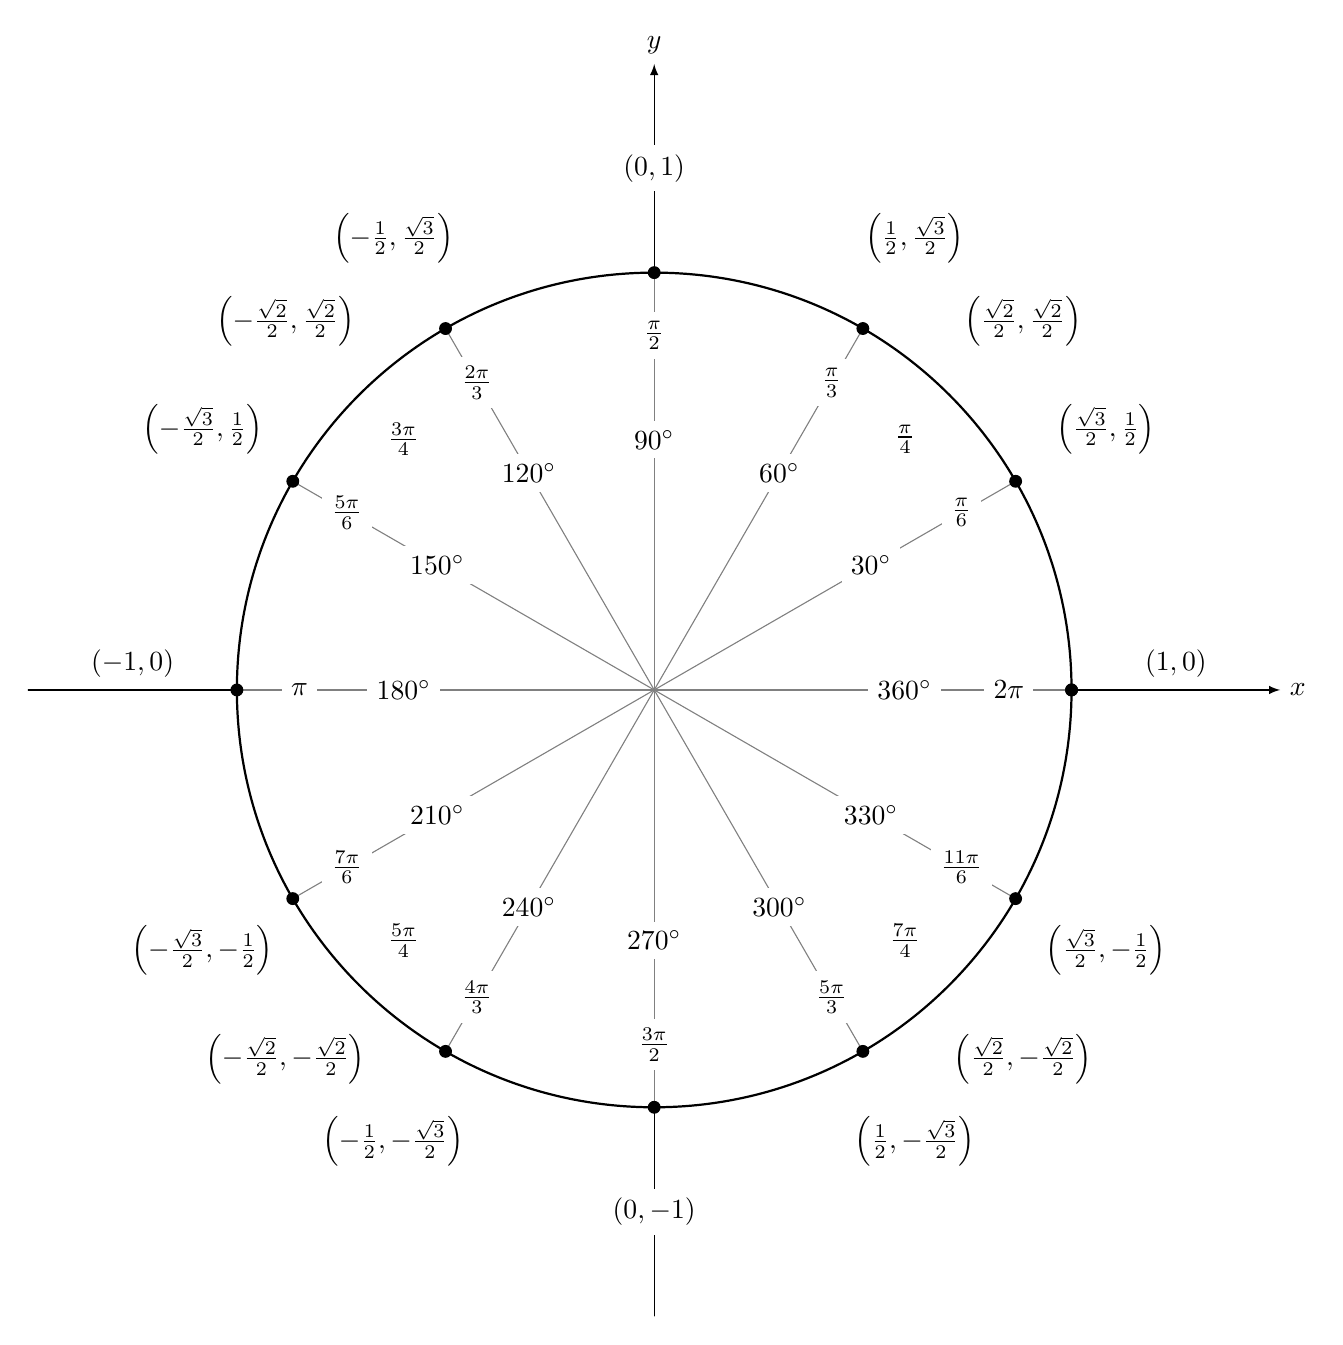
\begin{tikzpicture}[scale=5.3,cap=round,>=latex]
        % draw the coordinates
        \draw[->] (-1.5cm,0cm) -- (1.5cm,0cm) node[right,fill=white] {$x$};
        \draw[->] (0cm,-1.5cm) -- (0cm,1.5cm) node[above,fill=white] {$y$};

        % draw the unit circle
        \draw[thick] (0cm,0cm) circle(1cm);

        \foreach \x in {0,30,...,360} {
                % lines from center to point
                \draw[gray] (0cm,0cm) -- (\x:1cm);
                % dots at each point
                \filldraw[black] (\x:1cm) circle(0.4pt);
                % draw each angle in degrees
                \draw (\x:0.6cm) node[fill=white] {$\x^\circ$};
        }

        % draw each angle in radians
        \foreach \x/\xtext in {
            30/\frac{\pi}{6},
            45/\frac{\pi}{4},
            60/\frac{\pi}{3},
            90/\frac{\pi}{2},
            120/\frac{2\pi}{3},
            135/\frac{3\pi}{4},
            150/\frac{5\pi}{6},
            180/\pi,
            210/\frac{7\pi}{6},
            225/\frac{5\pi}{4},
            240/\frac{4\pi}{3},
            270/\frac{3\pi}{2},
            300/\frac{5\pi}{3},
            315/\frac{7\pi}{4},
            330/\frac{11\pi}{6},
            360/2\pi}
                \draw (\x:0.85cm) node[fill=white] {$\xtext$};

        \foreach \x/\xtext/\y in {
            % the coordinates for the first quadrant
            30/\frac{\sqrt{3}}{2}/\frac{1}{2},
            45/\frac{\sqrt{2}}{2}/\frac{\sqrt{2}}{2},
            60/\frac{1}{2}/\frac{\sqrt{3}}{2},
            % the coordinates for the second quadrant
            150/-\frac{\sqrt{3}}{2}/\frac{1}{2},
            135/-\frac{\sqrt{2}}{2}/\frac{\sqrt{2}}{2},
            120/-\frac{1}{2}/\frac{\sqrt{3}}{2},
            % the coordinates for the third quadrant
            210/-\frac{\sqrt{3}}{2}/-\frac{1}{2},
            225/-\frac{\sqrt{2}}{2}/-\frac{\sqrt{2}}{2},
            240/-\frac{1}{2}/-\frac{\sqrt{3}}{2},
            % the coordinates for the fourth quadrant
            330/\frac{\sqrt{3}}{2}/-\frac{1}{2},
            315/\frac{\sqrt{2}}{2}/-\frac{\sqrt{2}}{2},
            300/\frac{1}{2}/-\frac{\sqrt{3}}{2}}
                \draw (\x:1.25cm) node[fill=white] {$\left(\xtext,\y\right)$};

        % draw the horizontal and vertical coordinates
        % the placement is better this way
        \draw (-1.25cm,0cm) node[above=1pt] {$(-1,0)$}
              (1.25cm,0cm)  node[above=1pt] {$(1,0)$}
              (0cm,-1.25cm) node[fill=white] {$(0,-1)$}
              (0cm,1.25cm)  node[fill=white] {$(0,1)$};
\end{tikzpicture}


\newpage

\begin{multicols}{2}
\textbf{Sats:}\par
\begin{align*}
  &360^\circ = 2\pi rad \\
  &v_{g} = v_{r} \cdot \frac{180^\circ}{\pi} \\
  &v_{r} = v_{g} \cdot \frac{\pi}{180^\circ} \\
\end{align*}

\textbf{Sats:}\par
\begin{align*}
  &-1 \leq \sin{t} \leq 1 \\
  &-1 \leq \cos{t} \leq 1 \\
\end{align*}

\textbf{Sats:}\par
\begin{align*}
  &\cos{(-t)} = \cos{(t)} \\
  &\sin{(-t)} = -\sin{(t)} \\
  &\tan{(-t)} = \frac{\sin{(-t)}}{\cos{(-t)}} = \frac{-\sin{(t)}}{\cos{(t)}} \\
\end{align*}

\textbf{Additionsformlerna:}\par
\begin{align*}
  &\sin{(\alpha + \beta)} = \sin{(\alpha)}\cos{(\beta)} + \sin{(\beta)}\cos{(\alpha)} \\
  &\sin{(\alpha - \beta)} = \sin{(\alpha)}\cos{(\beta)} - \sin{(\beta)}\cos{(\alpha)} \\
  &\cos{(\alpha + \beta)} = \cos{(\alpha)}\cos{(\beta)} - \sin{(\beta)}\sin{(\alpha)} \\
  &\cos{(\alpha - \beta)} = \cos{(\alpha)}\cos{(\beta)} + \sin{(\beta)}\sin{(\alpha)} \\ 
\end{align*}

\textbf{Trigonometriska ettan:}\par
\begin{align*}
  &(\sin{t})^{2} + (\cos{t})^{2} = 1 \\
  &\sin^{2}{t} + \cos^{2}{t} = 1 \\ 
\end{align*}


\subsection{Exempel: Trigonometri}
\begin{align*}
  \begin{aligned} \cos \frac { \pi } { 12 } & = \cos \left( \frac { \pi } { 3 } - \frac { \pi } { 4 } \right) = \cos \frac { \pi } { 3 } \cos \frac { \pi } { 4 } + \sin \frac { \pi } { 3 } \sin \frac { \pi } { 4 } \\ & = \left( \frac { 1 } { 2 } \right) \left( \frac { 1 } { \sqrt { 2 } } \right) + \left( \frac { \sqrt { 3 } } { 2 } \right) \left( \frac { 1 } { \sqrt { 2 } } \right) = \frac { 1 + \sqrt { 3 } } { 2 \sqrt { 2 } } \end{aligned}
\end{align*}


\section{Gränsvärden}
\begin{align*}
  &\lim_{x\to x_0} f = L \land \lim_{x\to x_0} g = M \\
  &\Rightarrow \lim_{x\to x_0}(f+g) = L+M  \\
  &\text{Squeeze therum: } h(x) \leq f(x) \leq g(x), \\
  &\lim_{x\to x_0} h(x) = \lim_{x\to x_0} g(x_0) = L \\
  &\Rightarrow \lim_{x\to x_0} f(x) = L \\
  &\lim_{x\to 0} \frac{\sin(x)}{x}=1  \\
  &\lim_{x\to\infty} \sin(x) \text{ är ej definerad}
\end{align*}


\textbf{Example: Limit för sin}
\begin{align*}
  &\text{Lös: } \lim_{x\to 0} \frac{\sin(2x^2)}{x^2}  \\
  &\lim_{x\to 0} \frac{2 \cdot \sin(2x^2)}{2x^2} = 2 \cdot \lim_{x\to 0} \frac{\sin(2x^2)}{2x^2} = 2
\end{align*}

\textbf{Example: 0/0}
\begin{align*}
  &\text{Lös: } \lim_{x\to 0} \frac{x \cdot \left( \cos(x) + \frac{\sin(x)}{x} \right) }{x+x^2} \\
  &\lim_{x\to 0} \frac{ x \cdot \left( \cos(x) + \frac{ \sin(x) }{ x } \right) }{x(1+x)} = \frac{1+1}{1} = 2  \\
\end{align*}

\textbf{Example: roten ur i nämnaren}
\begin{align*}
  &\text{Lös: } \lim_{x\to 0} \frac{x}{\sqrt{x+9}-3}  \\
  &\lim_{x\to 0} \frac{x(\sqrt{x+9}+3)}{(\sqrt{x+9}-3)(\sqrt{x+9}+3)} \\
  &=\lim_{x\to 0} \frac{x(\sqrt{x+9}+3)}{x+9-9} = \lim_{x\to 0} \sqrt{x+9}+3 = 6 \\
\end{align*}

\textbf{Example: roten ur i nämnaren}
\begin{align*}
  &\text{Lös: } \lim_{x\to-\infty} \frac{2x-1}{\sqrt{3x^2+x+1}}  \\
  &\lim_{x\to-\infty} \frac{x(2-\frac{1}{x})}{\sqrt{x^2(3+\frac{1}{x}+\frac{1}{x^2})}} \\
  &=\lim_{x\to-\infty} \frac{x(2-\frac{1}{x})}{x\sqrt{3+\frac{1}{x}+\frac{1}{x^2}}} = \frac{-2}{\sqrt{3}} \\
\end{align*}

\textbf{Example: infinity sin and squeeze}
\begin{align*}
  \text{Lös: } &\lim_{x\to\infty}\frac{\sin(x)}{x}  \\
  &\\
  |\frac{\sin(x)}{x}| &= \frac{|\sin(x)|}{|x|} \leq \frac{1}{|x|} \\
  &\Rightarrow \text{ squeeze } \lim_{x\to\infty}|\frac{\sin(x)}{x}| = 0  \\
  &\Rightarrow \lim_{x\to\infty}\frac{\sin(x)}{x} = 0  \\
\end{align*}


\subsection{Kontinuitet}
En funktion är kontnuelig i punkt $x_0, \; \forall \varepsilon \land \exists \delta: |x-x_0| < \delta \Leftrightarrow |f(x)-f(c_0)|<\varepsilon$.
Alltså så finns det inga hopp i funktionen. Man kan dra penan på grafen utan att släppa 
om functionen bestor av flera utryck är funktionen kontenuerlig om alla utrycken är det.


\section{Derivator}
\begin{itemize}
  \item Tangent: linjen som har samma lutining i en punkt som functionens derivata
  $y-f(x_0)=f'(x_0)(x-x_0) \Rightarrow y=ax+b$ %y-f(x_0)=f'(x_0)(x-x_0)
  \item Samband: Deriverbar $\Rightarrow$ Kontinuerlig
\end{itemize}

\textbf{Räkneregler}
\begin{center}
\begin{tabular}{ |c|c| } 
 \hline
 $f$       & $f'$         \\
 \hline
 $c$       & $0$          \\
 $x$       & $1$          \\ 
 $x^n$     & $nx^{n-1}$    \\  
 $a^x$     & $a^x\ln{a}$   \\ 
 $e^{kx}$  & $ke^{x}$       \\
 $\sin{x}$ & $\cos{x}$     \\
 $\cos{x}$ & $-\sin{x}$    \\
 $\tan{x}$ & $\frac{1}{\cos^2{x}}$    \\
 $\ln{x}$  & $\frac{1}{x}$ \\
 \hline
\end{tabular}
\end{center}

\begin{align*}
  &\quad  (f+g)' = f' + g' \\
  &\quad  (cf)'  = cf' \\
  &\quad  (fg)'  = f'g + fg' \text{ Produktregeln} \\
  &\quad  \left( \frac{f}{g} \right)' = \frac{f'g - fg'}{g^2} \text{ Kvotregeln, } g \neq 0 \\
\end{align*}

% derivatans Definetion
% flertal exemplel med squeeze, modifiering(0/0), sin
% tangent

\subsection{Kjedje regeln}
\begin{align*}
  &\text{Om functionen $f$ är deriverbar i $x$ och funktionen är} \\
  &\text{deriverbar i} g(x) \\
  &\Rightarrow h(x)=f \circ g = f(g(x)) \text{ deriverbar i } x \\
  &h'(x)=(f(g(x)))'=f'(g(x))g'(x)
\end{align*}

  \textbf{Example: Kjedje regeln}
  \begin{align*}
    &\text{Lös: } (x^x)'  \\
    &(x^x)'=\left( e^{x\ln{x}} \right)'=e^{x\ln{x}} \left( \ln{x}+x\frac{1}{x} \right) \\
    &= e^{x\ln{x}}(1+\ln{x})=x^x(1+\ln{x}) \\
  \end{align*}


  \subsection{L'Hôpital's rule} 
  \begin{align*}
    &f,g:\mathbb{R}\to\mathbb{R} \land \left( \lim_{x \to x_0}\frac{f}{g}
    =\frac{0}{0}\lor ''{\lim_{x\to x_0}\frac{f}{g}=\frac{\pm \infty}{\pm \infty}}'' \right) \\
    &\Rightarrow \lim_{x \to x_0}\frac{f}{g}=\lim_{x \to x_0}\frac{f'}{g'} \\ 
  \end{align*}

  \textbf{Example: L'Hôpital's rule}
  \begin{align*}
    &\text{Lös: } \lim_{x \to 1}\frac{x^4-6x^3+5x^2}{x^3-8x^2+7x}\\
    &\lim_{x \to 1}\frac{x^4-6x^3+5x^2}{x^3-8x^2+7x} = '' \; \frac{0}{0} \; '' \\
    &\text{L'Hôpital's rule} \Rightarrow \lim_{x \to 1}\frac{4x^3-18x^2+10x}{3x^2-16x+7} \\
    &= \frac{-4}{-6} = \frac{2}{3} \\
  \end{align*}


  \subsection{Medelvärdessatsen} 
  \begin{align*}
    &\text{Anta att $f$ är kontinuerlig på $[a,b]$ och deriverbar} \\
    &\text{på} (a,b) \Rightarrow \exists c \in (a,b) \\
    &\text{så att } \frac{f(b)-f(a)}{b-a}= f'(c)
  \end{align*}

  \textbf{Example: Medelvärdessatsen}
  \begin{align*}
    &\text{Bevisa att för varge $a>b$ gäller följande} \\
    &|\cos{a}-\cos{b}| \leq |a-b| \\
    &f(x)=\cos{x} \text{ är kont och deriverbar i } \mathbb{R} \land [ \, a,b ] \, \\
    &\text{MVS }\Rightarrow \exists c \in (a,b):f'(c)=\frac{f(b)-(a)}{b-a} \\
    &=\frac{\cos(b)-\cos(a)}{b-a}=-\sin(c) \\
    &\Rightarrow |\frac{\cos(b)-\cos(a)}{b-a}|=|-\sin(c)| \\
    &\Rightarrow \frac{|\cos(b)-\cos(a)|}{|b-a|}=|-\sin(c)| \leq 1 \\
    &\frac{|\cos(b)-\cos(a)|}{|b-a|} \leq 1 \\
    &\Rightarrow |\cos(b)-\cos(a)| \leq |a-b|
  \end{align*}


  \subsection{Rolle} 
  Anta att $f$ är kontinuerlig på $[a,b]$ och deriverbar på $(a,b)$. 
  Om $f(a)=f(b) \Rightarrow \exists c \in (a,b):f'(c)=0$.


  \subsection{växande funktioner}
  \begin{itemize}
    \item växande:          $x_1<x_2 \Rightarrow f(x_1) \leq f(x_2)$
    \item strängt växande:  $x_1<x_2 \Rightarrow f(x_1) < f(x_2)$
    \item avtagande:        $x_1<x_2 \Rightarrow f(x_1) \geq f(x_2)$
    \item stänkt avtagande: $x_1<x_2 \Rightarrow f(x_1) > f(x_2)$
  \end{itemize}


  \subsection{Högreordnings devivator}
  \begin{itemize}
    \item andragrads derivator:   $(f')' = f''  =\frac{d^2f}{dx^2}$
    \item tredjegrads derivator:  $(f'')'= f''' =\frac{d^3f}{dx^3}$
    \item ntegrads derivator:     $f^{(n)}= f^{n}=\frac{d^{n}f}{dx^{n}}$
  \end{itemize}


  \subsection{Impericit derivering}
  Deriverar båda sidorna om modifierat.

  \textbf{Example: Impericit derivering}
  \begin{align*}
    &\text{Bestäm tangenten till } x^3+y^3=6xy \; i \; (3,3) \\
    &(3^3+3^3=6\cdot3\cdot3) \text{ -sant} \\
    &y-y_0=f'(x_0)(x-x_0) \Rightarrow y-3=f'(3)(x-3) \\
    &\text{Implicit derivering: } 3x^2+3y^2y'=6y+6xy' \\
    &\Rightarrow 3x^2y'-6xy'=6y-6x^2 \\
    &\Rightarrow y'(3x^2-6x)=6y-3x^2
    \Rightarrow y'=\frac{6y-3x^2}{3x^2-6x} \\
    &\Rightarrow y'(3)=\frac{63-3\cdot3^2}{3\cdot3^2-6\cdot3}=-1 \\
    &\Rightarrow y-3=-(x-3) \\
    &\Rightarrow x+y=6 \lor y=-x+6 \\
  \end{align*}


  \subsection{invers funktioner} 
  \begin{align*}
    & f: A \to B \land Bijektiv \Rightarrow f^{-1}(x) \text{ Finns, där}  \\
    &\text{(1) }  x = f^{-1}(y) \Leftrightarrow y = f(x) \\
    &\text{(2) }  D_{f^-1} = V_f \Leftrightarrow D_f = V_{f^-1} \\
    &\text{(3) }  x = f^{-1}(f(x)), x \in D_f = V_{f^-1} \\ 
    &\text{(3) }  y = f^{-1}(f(y)), y \in D_f = V_{f^-1} \\ 
  \end{align*}

  % exempel

  \subsection{exponetial och logaritm}  % kolla om det är något nytt
  \begin{align*}
    &{\frac{a}{b}}^{-3} = {\frac{b}{a}}^{3} \\
    &\sqrt{a} = a^{\frac{1}{2}} \\
    &a^{x+y}=a^{x}a^{y} \\
    &{(a^{x})}^y=a^{xy} \\
    &a^{-x}=\frac{1}{a^x} \\
    &a^{\frac{m}{n}}={\sqrt{a^{m}}}^{n} \\
    & \\
    &\text{(1): } b = a^x \Leftrightarrow \log_a(b) \\
    &= x  \text{ för: } a>0, b>0, a \ne 1  \\
    &\text{(2): } \log_a(\frac{b}{c}) = \log_a(b) - \log_a(c) \\
    &\text{(3): } \log_a(b \cdot c) = \log_a(b) + \log_a(c) \\
    &\text{(4): } \log_a(b^d) = d\log_a(b) \\
    &\text{(5): } \log_a(b) = \frac{\log_f(b)}{\log_f(a)} \\
    &\text{(6): } \log_a(a) = 1 \\
    &\text{(7): } \log_a(1) = 0 \\
    &\text{(8): } a^{\log_a(x)} = x \\
    &\text{(9): } \log_{a^c}(b) = \frac{1}{c} \log_a(b) \\
  \end{align*}

  % exempel


  \subsection{odefinerad form}
  \begin{align*}
    &\quad  \frac{0}{0},\infty\cdot{0},1^{\infty},\infty^0,0^0 \\
  \end{align*}


  \subsection{inversa trigometriska funktioner}
  \subsubsection{arcsin}
  \begin{align*}
    &\cos: [\frac{-\pi}{2},\frac{\pi}{2}] \to [-1,1] \\
    &\arcsin{1}=\frac{\pi}{2} \\
    &\arcsin{0}=0 \\
    &\arcsin{\pi}=\text{odefinerad} \\
    &\sin(\arcsin(x))=x \\  
    &\arcsin(\sin(x))=x \\
    &(\arcsin(x))'=\frac{1}{\sin'(\arcsin(x))}=\frac{1}{\cos(\arcsin(x))} \\
    &=\frac{1}{\sqrt{\cos^2(\arcsin(x))}}=\frac{1}{\sqrt{1-\sin^2(\arcsin(x))}}=\frac{1}{\sqrt{1-x^2}} \\
  \end{align*}

  \subsubsection{arccos}
  \begin{align*}
    &\cos: [0,\pi] \to [-1,1] \\
    &\arccos{1}=0 \\
    &\arccos{0}=\frac{\pi}{2} \\
    &\arccos{\pi}=\text{odefinerad} \\
    &\cos(\arccos(x))=x \\  
    &\arccos(\cos(x))=x \\
    &(\arccos(x))'= \frac{1}{\sqrt{1-x^2}} \\
  \end{align*}

  \subsubsection{arctan}
  \begin{align*}
    &\cos: [\frac{-\pi}{2},\frac{\pi}{2}] \to \mathbb{R} \\
    &\tan(\arctan(x))=x \\  
    &\arctan(\tan(x))=x \\
    &(\arctan(x))'= \frac{1}{1+x^2} \\
  \end{align*}

  \subsubsection{exempel}
  \begin{align*}
    &\tan{(\arccos{x})} = \frac{\sin{(\arccos{x})}}{\cos{\arccos{x}}}= \frac{\sqrt{1-x^2}}{x} \\
    &\cos{(\arctan{x})} = \cos{\frac{\arcsin{x}}{\arccos{x}}}= \frac{1}{1+x^2} \\ %not corect steps4
    &\sin{(\arccos{x})} = \sqrt{1-x^2} \\
    &\cos{(\arcsin{x})} = \sqrt{1-x^2} \\
  \end{align*}


  \section{Grafritning}
  Ta reda på extrem punkterna och rita utifrån det

  \textbf{Extremvärden}
  \begin{align*}
    &\text{global minimum punkt: } x_0, \; \forall x: f(x) \geq f(x_0) \\
    &\text{lokal minimum punkt: } x_0, \; \forall x \text{ nära } x_0: f(x) \geq f(x_0) \\
    &\text{global maximum punkt: } x_0, \; \forall x: f(x) \leq f(x_0) \\
    &\text{lokal maximum punkt: } x_0, \; \forall x \text{ nära } x_0: f(x) \leq f(x_0) \\
    &\text{Kritisk punkt: } f'(x)=0 \\
  \end{align*}


  \textbf{Komplexity}
  \begin{itemize}
    \item konvex: Tangent liger altid under funktionen $y''>0$.
    \item konkav: Tangent liger altid över funktionen $y''<0$.
    \item Inflektionspunct: då funktionen byter från konvex till konkav eller tvärtom.
  \end{itemize}


  \textbf{Exemple: Datan som behövs beräknas vid grafritning}
  \begin{align*}
    &\text{Rita functionen } y={(x^2-1)}^3 \\
    &\text{(1) Kollar om functionen är Konternuelig:} \\
    &\text{Eftersom funkrionen består av polynom är} \\
    &\text{den konternuerlig}   \\
    &\text{(2) Extrem punkter: }   \\
    &\text{ (I) Derivatan: functionen är deriverbar } \\
    &y'=3{(x^2-1)}^2 \cdot 2x=0 \\
    &\Rightarrow x=0  \\
    &\text{ (II) Singulär punkter:} \\
    &\text{ eftersom funktionen är deriverbar i alla} \\
    &\text{ punkter i definitions mängden } \\
    &\text{ Så funns det inga singulär punkter} \\
    &\text{ (III) End värden: Eftersom funktionen är ej} \\
    &\text{ definerad i ett intervall så finns det inga} \\
    &\text{(3) Komplexitet: } \\
    &\text{Andra derivatan avgör om funktionen är} \\
    &\text{knvex eller konkav} \\
    &y''=(6x{(x^2-1)}^2)'= (6x{(x^4-2x^2+1)})' \\
    & = (6x^5-12x^3+6x)' = 30x^4-36x^2+6 = 0 \\
    &\Rightarrow t^2-\frac{6}{5}t+\frac{1}{5}=0 \\
    &\Rightarrow t=\frac{6}{10}\pm
    \sqrt{\frac{36}{100}-\frac{20}{100}} = \frac{6}{10} \pm \frac{4}{10}  \\
    &t=1 \lor t=\frac{1}{5} \Rightarrow x=\pm1 \lor x=\pm\frac{1}{\sqrt{5}}  \\
    &\text{(4) Asymptoter: } \\
    &\text{ (I) lodräta asymptoter: }  \\
    &\lim_{x->+\infty}y=+\infty \\
    &\lim_{x->-\infty}y=+\infty \\
    &\text{ (II) vågräta asymptoter:} \\
    &\text{Eftersom funktionen inte är en kvot finns} \\
    &\text{det inga sådana asymptoter }  \\
  \end{align*}
\end{multicols}
\raggedcolumns


  \begin{center}
  \begin{tabular}{ |c|c|c|c|c|c| } 
  \hline
          & $x<-1$    & $x=-1$            & $-1<x<-\frac{1}{\sqrt{5}}$ & $x=-\frac{1}{\sqrt{5}}$ & $\dots$ \\ 
  $f'$   & $-$       & $-$               & $-$                        & $-$                     & $\dots$ \\ 
  $f''$  & $-$       & $0$               & $+$                        & $0$                     & $\dots$ \\
  $f$    & avtagande & avtagande         & avtagande                  & avtagande               & $\dots$ \\
          & kokav     & inflektions punkt & konvex                     & inflektions punk        & $\dots$ \\
  \hline
  \end{tabular}
  \end{center}

\newpage
\begin{multicols}{2}
\section{Optemering}
Sats: om funktionen $f(x)$ är knternuerlig på det slutna intervalet $[a,b]$
så antar det sitt största värde och minsta värde där $\exists x_1,x_2\in[a,b]$
så att $f(x_1) \leq f(x) \leq f(x_2)$.


\textbf{Exempel: Max/Min värde}
\begin{align*}
  &\text{Låt } f(x):[-1,2]\to\mathbb{R}, f(x)=x^3-3|x|  \\
  &\text{(1) Konternuelig: } \\
  &\text{f är konternuerlig i intervallet}   \\
  &\\
  &\text{(2) Extrem punkter: }   \\
  &\text{ (I) Derivatan: functionen är deriverbar i} \\
  &\text{intervalet förutom då } x=0 \\
  &\text{låt f bestå av } f_1(x)=x^3-3x, x \geq 0 \\ 
  &\land f_1(x)=x^3+3x, x<0 \\
  &\Rightarrow f'_1(x)=3x^2-3, x \geq 0 \land f'_2(x)=3x^2+3, x<0 \\
  & f'_1(x)=0 \Rightarrow x=1 \in [1,2], f(1)=-2  \\
  & f'_2(x)=0 \Rightarrow x= \text{Odefinerad} \\
  &\text{ (II) Singulär punkter:} \\
  &\text{f är inte deriverbar då } x=0, f(0)=0 \\
  &\text{ (III) End punkterna: Eftersom funktionen är ej} \\
  &\text{definerad i ett intervall så finns det inga } \\
  &f(-1)=-4 \\
  &f(2) = 2 \\
  &\\
  &\text{(3) Största och minsta värdet: } \\
  &f(-1)<f(1)<f(0)<f(2)  \\
  &\text{Svar: Max är $2$, min är $-4$}  \\
\end{align*}


\section{Talfölder och serier}
\textbf{Def: Talföljder}
\begin{align*}
  &\text{En talföljd är en funktion } a:\mathbb{N}\to\mathbb{N}  \\
  &\text{Vi skriver $a_n$ istället för $a(n)$, $a_2=a(2)$} \\
  &\text{Vi säger att $a_n\to{a}\in\mathbb{N}$ så är den \textbf{konvergent}} \\
  &\text{Vi säger att $a_n\to\infty$ så är den \textbf{divergent} eller ej} \\
  &\text{existerande} \\
  &\text{Konvergent kan vara begränsad uppåt eller nedåt} \\
  &\text{Talföljed kan vara växande eller avtagande} \\
  &\\
  &a_n\to{a}\lor{b_n\to{b}} \\
  &\text{ Omm $a$ och $b$ existerar } a_n+b_n\to{a+b} \\
\end{align*}

\textbf{Exempel: Derivatan av serier}
\begin{align*}
  &\quad  \text{Ange } f'(2), \; f(x)= \displaystyle\sum_{n=1}^{\infty} \frac{{(x-2)}^n}{n^2 2^{2n}} \\
  &\quad  \text{Anger den första termen } \left( \frac{x-2}{4} \right)' = \frac{1}{4} \\
  &\quad  f'(x) = \frac{1}{4} + \displaystyle\sum_{n=2}^{\infty} \frac{n{(x-2)}^{n-1}}{n^2 2^{2n}}
  \text{ Inre och yttre derivatan} \\
  &\quad  f'(2) =  \frac{1}{4} + \displaystyle\sum_{n=2}^{\infty} \frac{n{(2-2)}^{n-1}}{n^2 2^{2n}}
  = \frac{1}{4} + 0 = \frac{1}{4} \\
\end{align*}


\textbf{Sats: }
Om ${(a_n)}^{\infty}$ är Konvergent $\Rightarrow (a_n), \; n=1$ är begränsad

  \textbf{Sats: }
  \begin{align*}
    &\quad  \text{Låt } a>0  \\
    &\quad  \text{ (I) } a^n\to{0} \text{ om } a<1 \\
    &\quad  \text{(II) } a^n\to{+\infty} \text{ om } a>1 \\
    &\quad  {{(a_n)}_{n=1}}^{\infty}=\displaystyle\sum_{k=0}^{n}a_n=a_1+a_2+a_3+\ldots \\
  \end{align*}

  \textbf{Sats: Geometrisk serie}
  \begin{align*}
    &\quad  s _ { n } = a + a k + a k ^ { 2 } + \ldots + a k ^ { n - 1 } = \frac { a \left( k ^ { n } - 1 \right) }
    { k - 1 } \\
    &\quad  \displaystyle\sum_{n=0}^{\infty}r^n \Rightarrow \\
    &\quad  \text{ Konvergent om } |r|<1  \\
    &\quad  \text{ divergent om } |r|<1  \\
  \end{align*}

\textbf{Sats: }
\begin{align*}
  &\quad  \displaystyle\sum_{n=0}^{\infty}a_n \text{ konvergent } \Rightarrow a_n\to{0} \\
\end{align*}

\textbf{Sats: p-serie}
\begin{align*}
  &\quad  \displaystyle\sum_{n=0}^{\infty}\frac{1}{n^p} \Rightarrow \\
  &\quad  \text{ konvergent om } \Rightarrow p>1 \\
  &\quad  \text{ divergent om } \Rightarrow p\leq1 \\  
\end{align*}

\textbf{Sats: }
\begin{align*}
  &\quad  \text{Antag att } 0 \leq a_n \leq b_n \text{ för varge } n\in \mathbf{N} \\
  &\quad  \displaystyle\sum_{n=1}^{\infty}a_n \text{ konvergent } \Rightarrow a_n\to{0} \\
  &\quad  (I) \displaystyle\sum_{n=1}^{\infty}b_n \text{ konvergerar}
  \Rightarrow \displaystyle\sum_{n=1}^{\infty}a_n \text{ konvergerar} \\
  &\quad  (II) \displaystyle\sum_{n=1}^{\infty}a_n \text{ derigerar}
  \Rightarrow \displaystyle\sum_{n=1}^{\infty}b_n \text{ derigerar} \\
\end{align*}

% exempel

\textbf{Sats: }
\begin{align*}
  &\text{Antag att } a_n >0, \; b_n >0 \text{ för varje } n \in \mathbf{N} \\
  &\text{ och antag att } \frac{a_n}{b_n}\to L \neq 0 \; \land L < \pm\infty\\
  &\text{Då gäller att serien } \displaystyle\sum_{n=1}^{\infty}a_n \text{ och }
  \displaystyle\sum_{n=1}^{\infty}b_n \\
  &\text{är båda divergenta} \\
\end{align*}

\textbf{Sats: kvotkriterium}
\begin{align*}
  &\text{Låt } a_n>0 \land \lim_{n\to{\infty}}\frac{a_{n+1}}{a_n}\to L \Rightarrow \\
  &(I) \; 0 \leq L \leq 1 \Rightarrow \text{ Konvergerar } \displaystyle\sum_{n=1}^{\infty}a_n
  (a_n \to 0) \\
  &(II) \; L>1 \Rightarrow \displaystyle\sum_{n=1}^{\infty}a_n \text{ derigerar }
  (a_n \to +\infty) \\
\end{align*}

\textbf{Exemple: Måste kunna}
\begin{align*}
  &\displaystyle\sum_{n=1}^{\infty}\frac{5^n n!}{n^n} \\
  &\text{Låt } a_n = \frac{5^n n!}{n^n} \Rightarrow \frac{a_{n+1}}{a_n} =
  \frac{5^{n+1}(n+1)!/n^n}{5^n n!/n^n} \\
  &= 5 \frac{(n+1)n^n}{{(n+1)}^{n+1}} = 5 {(\frac{n}{n+1})}^n = \\
  &= 5 \frac{1}{{(1+1/n)}^n} \to \frac{5}{e} > 1 \Rightarrow \text{ derigerar}\\
\end{align*}


\textbf{Sats: Rotkriteriet (Ovanlig)}
\begin{align*}
  &\text{Låt } a_n>0 \land \lim_{n\to{\infty}}\sqrt[n]{a_n} \to L \Rightarrow \\
  &(I) \; 0 \leq L \leq 1 \Rightarrow \text{ Konvergerar } \displaystyle\sum_{n=1}^{\infty}a_n
  (a_n \to 0) \\
  &(II) \; L>1 \Rightarrow \displaystyle\sum_{n=1}^{\infty}a_n \text{ derigerar }
  (a_n \to +\infty) \\
\end{align*}

\subsection{Serier med varierande tecken}
\textbf{Sats: leibinz}
\begin{align*}
  &\text{Antag att } \displaystyle\sum_{n=1}^{\infty}a_n \text{ är en alternerande serie } \\
  &\text{och att om } |a_n| \to 0 \land |a_n|\geq|a_{n+1}| \Rightarrow konvergent \\
\end{align*}

\textbf{Def: absolut konvergent}
\begin{align*}
  &\text{Endast om } \displaystyle\sum_{n=1}^{\infty}|a_n| \text{ konvagerar } \\
  &\Rightarrow
  \text{ då är den absolutkonvergent} \\
  &\text{om seriern är absolutkonvergent så är den också} \\
  &\text{konvergent behöver inte vara tvärtom} \\
\end{align*}


% konvergens radien 
\subsection{Potensserier}
\textbf{Def: Potensserier}
\begin{align*}
  &\text{En potensserier kring $x_0$ är en serie på formen } \\
  &\displaystyle\sum_{n=1}^{\infty}a_n{(x-x_0)}^n, \; a_n \in \mathbb{R} \text{ (koefficienten)} \\
  &x \text{ är en variabel} \\
\end{align*}

\textbf{Def: Konvergens radie}
\begin{align*}
  &T(x)=\displaystyle\sum_{n=1}^{\infty}\frac{{f(x_0)}^{(n)}}{n!}{(x-x_0)}^n \\
  &\text{vid exempelvis grad 2 så blir det andra derivatan} \\
  &\text{man räknar ut} \\
  &R=L^{-1}=\frac{1}{L} \\
  &L \text{ är där serien konvergerar, R är konvergens radie} \\
  &\displaystyle\sum_{n=1}^{\infty}a_n{(x-x_0)}^n, \; a_n \in \mathbb{R} \text{ (koefficienten)} \\
  &x \text{ är en variabel} \\
  &\text{Om konvergens radien är noll så finns det inte} \\
  &\text{några intervar för konvergens eller divergens}
\end{align*}

\textbf{Sats: Potensserier}
\begin{align*}
  &\text{En potensserie kring } x_0 \text{ är en serie på formen } \\
  &\displaystyle\sum_{n=1}^{\infty}a_n{(x-x_0)}^n a_n \in \mathbb{R} a_n \text{ koficienten } x \\
  &\text{är en variabel} \\
  &\text{När det står ex } {(3x+2)}^n \text{ så måste det stå med i } \\
  &a_n, 3^n \\
\end{align*}

\textbf{Exempel: Potensserier}
\begin{align*}
  &\displaystyle\sum_{n=1}^{\infty}\frac{{(x-7)}^n}{n(n+1)} \text{ är en potensserie där } \\
  &x_0=7, a_n=\frac{1}{n(n+1)} \\
  &|\frac{a_{n+1}}{a_n}| = |\frac{1/((n+1)(n+2))}{1/(n(n+1))}| = |\frac{n}{n+2}| =
  |\frac{n}{n(1+2/n)}| \\
  &\Rightarrow |\frac{1}{1}| = 1, \text{ då } n \to \infty \\
  &\Rightarrow R=\frac{1}{1}=1 \Rightarrow \text{ vi får följande intervall av} \\
  &\text{potenserien} \\
  &\text{Absolutkonverget för } |x-7|<1 \Leftrightarrow 6<x<8 \\
  &\text{Divergent för } |x-7|>1 \Leftrightarrow 8<x \lor x<6 \\
  &\\
  &\text{Testar edge fallen } x=6, x=8 \\
  &\displaystyle\sum_{n=1}^{\infty}\frac{{(8-7)}^n}{n(n+1)} 
  \Rightarrow |\displaystyle\sum_{n=1}^{\infty}\frac{{(1)}^n}{n(n+1)}|, \\
  &|\frac{{(1)}^n}{n(n+1)}|\to0 \Rightarrow \text{ absolutkonvergerar} \\
  &\displaystyle\sum_{n=1}^{\infty}\frac{{(6-7)}^n}{n(n+1)} 
  \Rightarrow |\displaystyle\sum_{n=1}^{\infty}\frac{{(-1)}^n}{n(n+1)}|, \\
  &|\frac{{(-1)}^n}{n(n+1)}|\to0 \Rightarrow \text{ absolutkonvergerar} \\
  &\\
  &\text{\textbf{Svar:} } \\
  &\text{Absolutkonverget för } 6\leq x\leq 8 \\
  &\text{Divergent för } 8<x \lor x<6 \\
\end{align*}


\subsection{Taylor serier}

\textbf{Def: Talorpolynom}
\begin{align*}
  &\text{Taylorpolynom av grad } n \in \mathbb{N}, \; kring \; x=x_0 \\
  &f(x)=P_n(x)= \displaystyle\sum_{k=0}^{n}\frac{f^{(k)}(x_0)}{k!}{(x-x_0)}^k, \; 0!=1,f^{(0)}=f \\
  &\text{När } x \approx x_0 \Rightarrow f(x) \approx p_n(x) \\
\end{align*}

\textbf{Sats: Talor sats}
\begin{align*}
  &\text{Antag att $f\in c^{n+1}$.} \\
  &f(x)=p_n(x)+R_{n+1}(x) \text{ Där felet är } R_{n+1}(x) \\
  &R_{n+1}(x)=\frac{f^{(n+1)}(c)}{(n+1)!}{(x-x_0)}^{n+1}, \; x \lor x_0 \leq c \leq x_0 \lor x \\
\end{align*}

\textbf{exempel: felet}
\begin{align*}
  &\text{Upskata felet hos } f(x)=\sin{x}, \text{ med grad } 5 \\
  &\\
  &\text{Sista termen är } \frac{x^5}{5!} \Rightarrow \text{Felet } \frac{f^{(6)}(c)}{6!}x^6, (0<c<1) \\
  &\left| \frac{f^{(6)}(c)}{6!}x^6 \right| \leq \frac{|f^{(6)}(c)|}{6!} = \frac{|\sin{c}|}{6!}
  \leq \frac{1}{6!} = \frac{1}{720} \\
\end{align*}

% calculate error example

\textbf{Exempel: grad n vid specificerad punkt}
Lös: Hitta Taylorpolynomet, ording $2n-1$, \text{ för } $\sin{2x}$ \text{ vid } $x=\frac{\pi}{2}$ \\
\begin{center}
  \begin{tabular}{ p{3cm} p{1cm} }
   $f(x)=\sin(2x)$ & $f(\frac{\pi}{2})=0$ \\ 
   $f'(x)=-2\cos(2x)$ & $f(\frac{\pi}{2})=-2$ \\ 
   $f''(x)=-2^2\sin(2x)$ & $f(\frac{\pi}{2})=0$ \\ 
   $f^{(3)}(x)=-2\cos(2x)$ & $f(\frac{\pi}{2})=2^3$ \\ 
   $f^{(4)}(x)=-2^2\sin(2x)$ & $f(\frac{\pi}{2})=0$ \\ 
   $f^{(5)}(x)=-2^4f'(x)$ & $f(\frac{\pi}{2})=-2^5$ \\ 
   $p_{2n-1}(x)=-2(x-\frac{\pi}{2})$  & \\ 
   $+\frac{2^3}{3!}{(x-\frac{\pi}{2})}^3$ & \\ 
   $-\frac{2^5}{5!}{(x-\frac{\pi}{2})}^5+\ldots$ & \\ 
   $+\frac{{(-1)}^n\cdot2^{2n-1}}{(2n-1)!}{(x-\frac{\pi}{2})}^{(2n-1)}$ & \\ 
  \end{tabular}
\end{center}


\textbf{Def: maclaurin polynomial}
\begin{align*}
  &\text{Taylorpolynom av grad } n \in \mathbb{N}, \text{ då } x_0=0 \\
  &\text{Big-O notation: Vi säger att} g(x)=O(f(x)) \\
  &\text{när } x \approx x_0, \text{ värsta fall} \\
  &\text{Man kan också säga istället för Big-O notation en rest} \\
  &R_{n+1}(x)=x^{n+1}H(x) \text{ där } H(x) \text{ begränsad i intervalet} \\
  &e^x=\displaystyle\sum_{k=0}^{n}\frac{x^k}{k!}+O(x^{n+1}) \\
  &\sin{x}=\displaystyle\sum_{k=0}^{n}\frac{{(-1)}^{k-1}}{(2k-1)!}x^{2k-1}+O(x^{2n}) \\
  &\cos{x}=\displaystyle\sum_{k=0}^{n}\frac{{(-1)}^{k}}{(2k)!}x^{2k}+O(x^{2n+19}) \\
  &\ln{(1+x)}=\displaystyle\sum_{k=0}^{n}\frac{x^k}{k}{(x)}^x+O(x^{n+1}) \\
\end{align*}


\section{Integraler}

\textbf{Regler no.1}
\begin{align*}
  &\int_a^a f(x)dx=0  \\
\end{align*}

\textbf{Regler no.2}
\begin{align*}
  &\int_a^b f(x)dx = -\int_b^a f(x)dx  \\
\end{align*}

\textbf{Regler no.3 (Linjearitet)}
\begin{align*}
  &A,B \in \mathbb{R} \\
  &\int_a^b (A \cdot f(x) dx + B \cdot g(x)) \\
  &= A(\int_a^b f(x) dx) + B(\int_a^b g(x) dx) \\
  &\text{Fungerar på subtraction men INTE} \\
  &\text{multiplicatione eller divition!}
\end{align*}

\textbf{Regler no.4}
\begin{align*}
  &c \in [a,b] \\
  &\int_a^b f(x)dx = \int_a^c f(x)dx + \int_c^b f(x)dx \\
\end{align*}

\textbf{Regler no.5}
\begin{align*}
  &f(-x)=-f(x) \text{ är udda} \\
  &\int_{-a}^a f(x)dx = 0 \\
\end{align*}

\textbf{Regler no.6}
\begin{align*}
  &f(-x)=f(x) \text{ är jämn} \\
  &\int_{-a}^a f(x)dx = 2 \int_0^a f(x)dx \\
\end{align*}

\textbf{Regler no.7}
\begin{align*}
  &\left| \int_a^b f(x)dx \right| \leq \int_a^b |f(x)|dx \\
\end{align*}

\textbf{Regler no.8}
\begin{align*}
  &f(x) \leq g(x) \Rightarrow \int_a^b f(x)dx \leq \int_a^b g(x)dx \\
\end{align*}


\textbf{Sats: Medelvärdessatsen för integraler}
\begin{align*}
  &f:[a,b]\to\mathbb{R} \text{ konternuelig }\land\exists c\in(a,b) \\
  &\Rightarrow \int_a^{b}f(x)dx=f(c)(b-a) \\
\end{align*}

\textbf{Sats: Fanalysens huvudsats, Fundemetal theorem of calculus} \newline
Satsen är den vi andvänder för att lösa integraler utan geometrisk tolkning
\begin{align*}
  &f:[a,b]\to\mathbb{R} \text{ konternuelig } \\
  &\Rightarrow F(x)=\int_a^x f(t)dt, \; a\leq x\leq b \\
\end{align*}

\textbf{Sats: }
\begin{align*}
  &f:[a,b]\to\mathbb{R} \text{ konternuelig } \\
  &\Rightarrow F \text{ är e primitiv funktion till } f(F'(x)=f(x)) \\
  &\int_a^b f(x)dx=F(b)-F(a) \\
  &\text{Vi skriver } \int_a^b f(x)dx={{[F(x)]}_a}^b=F(b)-F(a) \\
\end{align*}

\textbf{Exempel: arean mellan två grafer}
\begin{align*}
  &\int_a^b (f(x)-g(x))dx \text{ där f är översta} \\
  &\text{funnktionen och g är understa} \\
  &\int_0^1 (x-x^2)dx={{[x^2/2-x^3/3]}_0}^1 \\
  &=1/2-1/3=1/6 \\
\end{align*}


\textbf{Primitiva funktioner (Obestämda integralen)}
\begin{center}
\begin{tabular}{ |c|c| } 
  \hline
  $\int f dx$             & $F$              \\
  \hline
 $\int 1dx$               & $x+c$            \\
 $\int n^n dx$            & $x^{n+1}/(n+1)+c$ \\ 
 $\int 1/x dx$            & $\ln{|x|}+c$     \\  
 $\int\sin{x}dx$          & $-\cos{x}+c$     \\ 
 $\int\cos{x}dx$          & $\sin{x}+c$      \\
 $\int e^x dx$            & $e^x+c$          \\
 $\int 1/\sqrt{1-x^2} dx$ & $\arcsin{x}+c$   \\
 $\int 1/(x^2+1) dx$      & $\arctan{x}+c$   \\ % ändrade - till +
 $\int 1/\cos^2{x} dx$    & $\tan{x}+c$      \\
 \hline
\end{tabular}
\end{center}

\textbf{Exempel: }
\begin{align*}
  &\int_a^b e^x dx = {{[e^x]}_a}^b = e^b-e^a \\
  &\int_ e^x dx=e^x + c, \; c \in \mathbb{R} \\
\end{align*}

% subsub medelvärdet
\textbf{Def: medelvärdet}
\begin{align*}
  &Avgf = \frac{1}{b-a} \int_a^b f dx \\
\end{align*}


\subsection{variabelsubstition}
% https://www.youtube.com/watch?v=IAh00vU3FSY&t=457s
\begin{align*}
  &\int f'(g(x))g'(x) dx = f(g(x))+c \\
  &\int_ e^x dx=e^x + c, \; c \in \mathbb{R} \\
\end{align*}

\textbf{Exempel: }
\begin{align*}
  &\int {e^x}^2 2x dx  \\
  &\text{Låt } u=x^2 \Rightarrow du=2x dx \Rightarrow \int {e^x}^2 2x dx=\int e^u du = \\
  &= e^u+c={e^x}^2+c, \; c\in\mathbb{R} \\
\end{align*}


\subsubsection{Integraller som följer mönster}

\begin{align*}
  &\text{Integralles som inehåller } \sqrt{x^2+a^2}, \; a > 0  \\ 
  &x=a\tan{u} \Rightarrow u=\arctan{x}, \; -\pi/2<u<\pi/2  \\
  &\Rightarrow \sqrt{x^2+ a^2}=\sqrt{a^2+a^2\tan^2{u}} \\
  &=\sqrt{a^2(1+\tan^2{u})} = a\sqrt{\frac{\sin^2{u}+\cos^2{u}}{\cos^2{u}}} = a \frac{1}{\cos{u}} \\
  &\\
  &\text{Exempel: } \int \frac{1}{{(1+25x^2)}^{3/2}}dx \\
  &\int \frac{dx}{\sqrt{1+25x^2}^3}=\int \frac{dx}{\sqrt{25(1/25+x^2)}^3} \\
  &=\frac{1}{5^3} \int \frac{dx}{\sqrt{1/205x^2}^3} \\
  &\text{Låt } x=1/5\tan{u} \Leftrightarrow u=\arctan{5x} \\
  &\Rightarrow dx=\frac{1}{5\cos^2{u}}du \\
  &\Rightarrow \frac{1}{5^3} \int \frac{dx}{\sqrt{1/205x^2}^3} \\
  &=\frac{1}{5^3}\int\frac{\cos^3{u}}{{1/5}^3}\frac{1}{5\cos^2{u}}du=\frac{1}{5}\int\cos{u}du \\
  &=\frac{1}{5}\sin{u}+c = \frac{1}{5}\sin{\arctan{5x}}+c \\
  &\text{ Kan nu förenkla med trigo regler} \\
  &\text{och få: } \frac{x}{\sqrt{1+25x^2}}+c \\
\end{align*}

\begin{align*}
  &\text{Integralles som inehåller } \sqrt{x^2-a^2}, \; a > 0  \\ 
  &x=\frac{a}{\cos{u}} \Rightarrow u=\arccos{\frac{a}{x}} \\
  &\Rightarrow \sqrt{x^2-a^2}=\sqrt{\frac{a^2}{\cos^2{u}}-a^2}=\sqrt{\frac{a^2-a^2\cos^2{u}}{\cos^2{u}}} \\
  &=\sqrt{\frac{a^2\sin^2{u}-a^2\cos^2{u}}{a^2\cos^2{u}}} = a|\tan{u}| \\
\end{align*}

\begin{align*}
  &\text{Integralles som inehåller } \sqrt{ax+b} \\ 
  &ax+b=u^2 \\
  &\\
  &\text{Exempel: } \int \frac{dx}{2+\sqrt{x}} \\
  &\text{Låt: } u^2=x \Rightarrow 2udu=dx \\
  &\Rightarrow \int\frac{2udu}{2+u} = 2\int\frac{u+2-2}{2+u}du = 2\left( \int du -2\int\frac{du}{2+u} \right) \\
  &= 2u -4(\ln{2+u}) +c \\
\end{align*}



\subsection{Integration av rationella funktioner}
Om det står beräkna generaliserade integrallen så ska man beräkna med detta
Rationella funktioner: $R(x)=\frac{P(x)}{Q(x)}, \; P,Q$ är polynom.

\textbf{Algoritm}
\begin{itemize}
  \item Polynom divition om grad av täljare är stören än grad av nämnare
  \item Faktorisera nämnaren i realla faktorer
  \item Partiella bråk och sedan integrera dem, (dela up i mindre lösbara integraller)
\end{itemize}

\textbf{Partiella bråk}

När nämnaren har en förstagradsfaktor med potens $(x-\alpha)^{n}$ så ansätts termerna.
\begin{align*}
  \frac{A_1}{x-\alpha} + \frac{A_2}{(x-\alpha)^2} + \ldots + \frac{A_n}{(x-\alpha)^n}
\end{align*}

Andragradsfaktor $(x^2+ax+b)^m$ get upphov till ansatsen
\begin{align*}
  \frac{B_1x+C_1}{x^2+ax+b} + \frac{B_2x+C_2}{(x^2+ax+b)^2} + \ldots + \frac{B_mx+C_m}{(x^2+ax+b)^m}
\end{align*}
\end{multicols}
\raggedcolumns

 
\begin{center}
\begin{tabular}{ |c|c| } 
  \hline
  $x-a$                     & $\frac{A}{x-a}$                                                  \\
  \hline
  ${(x-a)}^k$               & $\frac{A_1}{x-a}+\frac{A_2}{{x-a}^2}+\ldots+\frac{A_k}{{x-a}^k}$  \\
  \hline
  $x^2+bx+c, \; (b^2-4c<0)$ & $\frac{Ax+B}{x^2+bx+c}$                                           \\
  \hline
 $x^2+bx+c, \; (b^2-4c<0)$ & $\frac{A_1x+B_1}{x^2+bx+c}+\frac{A_2x+B_2}{{(x^2+bx+c)}^2}+\ldots+\frac{A_1x+B_1}{{(x^2+bx+c)}^k}$  \\
 \hline
\end{tabular}
\end{center}


\newpage
\begin{multicols}{2}
\begin{align*}
  &\quad  \int \frac{1}{ax+b}dx = \frac{1}{a} \ln{|ax+b|} +c \\
  &\quad  \int \frac{x}{x^2+a^2}dx = \frac{1}{2} \ln{|x^2+a^2|} +c \\
  &\quad  \int \frac{x}{x^2-a^2}dx = \frac{1}{2} \ln{|x^2-a^2|} +c \\
  &\quad  \int \frac{dx}{x^2+a^2} = \frac{1}{a} \tan^-1{\frac{x}{a}} +c \\
  &\quad  \int \frac{dx}{x^2-a^2} = \frac{1}{2a} \ln{\frac{x-a}{x+a}} +c \\
\end{align*}


\begin{align*}
  &\int \frac{x^3+2}{x^2-5x+4}dx \\
  &\\
  &\text{1. Polynomdivition} \\
  &P(x)=x^3+2, \; Q(x)=x^2-5x+4 \\
  &\text{Med polynom divition så får vi kvot} \\
  &x+5 \text{ och rest } 21x-18 \\
  &x^3+2=(x+5)(x^2-5x+4) + 21x-18 \\
  &\\
  &\text{2. Faktorisera nämnaren i realla faktorer} \\
  &\Rightarrow \int \frac{x^3+2}{x^2-5x+4}dx \\
  &= \int \frac{(x+5)(x^2-5x+4) + 21x-18}{x^2-5x+4}dx \\
  &\int (x+5)dx + \int \frac{21x-18}{x^2-5x+4} \\
  &\\
  &\text{3. Integrerar partiella bråk} \\
  &\frac{21x-18}{x^2-5x+4} = \frac{21x-18}{(x-4)(x-1)} = \frac{A}{x-4} + \frac{B}{x-1} \\
  &\Rightarrow \frac{21x-18}{(x-4)(x-1)} = \frac{Ax-A+Bx-4B}{(x-4)(x-1)} \\
  &\Rightarrow A+B=21 \land -A-4B=-18 \\
  &\Rightarrow A=22 \land B=-1 \\
  &\int (x+5)dx + \int \frac{22}{x-4}dx - \int \frac{1}{x-1}dx \\
  &\\
  &\text{Svar: } x^2/2 +5x +22\ln{|x-4|} -\ln{|x-1|} +c, \; c \in \mathbb{R} \\
\end{align*}



\subsection{Partiell integration}
Om det är integraler med två funktioner så hjälper oftast partiell integration

\textbf{Formel}
\begin{align*}
  &\int_a^b f'g dx={[fg]}_a^b-\int_a^b fg' dx \\
  &\int f'g dx= fg-\int fg' dx \\
\end{align*}

\textbf{Bevis}
\begin{align*}
  &(f(x)g(x))'=f'(x)g(x)+f(x)g'(x) \Rightarrow \\
  &\int_a^b (fg)' dx= \int_a^b f'g dx + \int_a^b fg' dx \\
  &\Rightarrow  \int_a^b f'g dx = \int_a^b (fg)' dx - \int_a^b fg' dx \\
  &\int_a^b f'g dx={[fg]}_a^b-\int_a^b fg' dx \\
\end{align*}


% polynom trignomotrik
\textbf{Exempel: polynom * trignomotrik}
\begin{align*}
  &\int_0^{\pi/2} x\sin{x} dx \\
  &\int_0^{\pi/2} (-\cos{x})'x dx = {[-x\cos{x}]}_0^{\pi/2}+\int_0^{\pi/2} \cos{x}(x)' dx  \\
  &={[-x\cos{x}]}_0^{\pi/2} + {[\sin{x}]}_0^{\pi/2}=1 \\
\end{align*}

% exponesiel och polynom   ex5
\textbf{Exempel: polynom * exponensiel}
\begin{align*}
  &\int e^x x^2 dx \\
  &\int (e^x)' x^2 dx = [e^x x^2] - \int e^x 2x dx = e^x x^2 - 2 \int (e^x)' x dx \\
  &= e^x x^2 - 2e^x x + 2\int (e^x)' dx = e^x x^2 - 2e^x x + 2e^x +c \\
\end{align*}

% exponensiel och trigometrisk   (e^x cosx) ex6  
\textbf{Exempel: exponensiel * trignomotrik}
\begin{align*}
  &\int e^x\cos{x} dx \\
  &\text{Låt } I = \int e^x\cos{x} dx = \int {(e^x)}'\cos{x} \\
  &= e^x\cos{x} - \int e^x\sin{x}dx = e^x\cos{x} + e^x\sin{x} \\
  &- \int e^x\cos{x}dx \Rightarrow I = e^x\cos{x}+e^{x}\sin{x}-I \\
  &\Rightarrow I = \frac{e^x\cos{x}+e^{x}\sin{x}}{2} + c
\end{align*}

% bonus  \ln{x}
\textbf{Exempel: bonus ln}
\begin{align*}
  &\int_1^2 \ln{x} dx \\
  &\int_1^2 x'\ln{x} dx = \ldots =2\ln{2}-1\\
\end{align*}



\subsection{Generaliserande integraler}
\textbf{Def: }
Antag att f är kontinuerlig i $a,b$ och att $\lim_{x \to a^+} f(x) = \infty$
Vi definerar den generaliserade integralen $\int_a^b f(x) dx$
$= \lim_{\varepsilon \to 0^+} \int_{a+c}f(x) dx$ ,,,,konstingst.
Om gränsvärdet existerar och är ändlig säger vi att integralen är konvergentn,
anart är den divergent.

\textbf{Betekning}
\begin{align*}
  &\varepsilon \text{ Andvänds för små tal }  \lim_{\varepsilon \to 0^+} \\
  &M \text{ Andvänds för stora tal } \lim_{M \to +\infty} \\
  &c \text{ Andvänds för konstanter } +c \\
\end{align*}

\textbf{Sats: }
\begin{align*}
  &\int_a^{+\infty} \frac{dp}{x^p}, \; a>0 \\
  &p > 1 \Rightarrow \text{ Konvergerar} \\
  &p \leq 1 \Rightarrow \text{ Divergerar} \\
\end{align*}

\textbf{Sats: Jämförelsesatsen}
\begin{align*}
  &\text{Anta att $f$ och $g$ är konternuerliga och } \\
  &0 \leq f(x) \leq g(x), ( a \in [ \, -\infty,+\infty ) \, , b \in ( \, -\infty,\infty ] \, ) \\
  &\text{(I) om integralen är konvergent } \int_a^b g(x)dx \\
  &\Rightarrow \int_a^b f(x)dx \text{ är också konvergent} \\
  &\text{(II) om integralen är divergent } \int_a^b f(x)dx \\
  &\Rightarrow \int_a^b g(x)dx \text{ är också divergent} \\
\end{align*}

\textbf{Sats: }
\begin{align*}
  &\text{Om $f(x)$ är positiv konternuerlig och avtagande i} \\
  &intervallet x\geq\mathbb{N}, \text{så är serien }  \displaystyle\sum_{n=N}^{\infty} f(n) \text{ konvergent} \\ 
  &\text{precis när  }  \int_N^{\infty} f(x)dx \text{ är konvergent} \\
\end{align*}

\textbf{Exempel: }
\begin{align*}
  &\text{Betämm om serien konvergerar eller divergerar} \\
  &\displaystyle\sum_{n=10}^{\infty} \frac{1}{n\ln{n}{(\ln{(\ln{n})})}^2} \\
  &f(x) = \frac{1}{x\ln{x}{(\ln{(\ln{x})})}^2} \\
  &\text{ är positiv, konternuerlig och avtagande då nämnaren} \\
  &\text{är stängt positivt ökande för } x \geq 10 \\
  &\int_{10}^{+\infty} f(x)dx = \lim_{M\to\mathbb{+\infty}} \int_{10}^{M} f(x)dx, \\
  &(u=\ln{\ln{x}} \Rightarrow du = 1/\ln{x} \cdot 1/x dx) 
  \Rightarrow \lim_{M\to+\infty} \int_{\ln{\ln{10}}}^{\ln{\ln{M}}} \frac{1}{u^2} \\
  &\lim_{M\to+\infty} {[-1/u]}_{\ln{\ln{10}}}^{\ln{\ln{M}}} \\
  &=\lim_{M\to+\infty} (-1/\ln{\ln{M}}+1/\ln{\ln{M}}) \\
  &=1/\ln{\ln{M}} \\
  &\displaystyle\sum_{n=10}^{\infty} \frac{1}{n\ln{n}{(\ln{(\ln{n})})}^2} \text{ konverger} \\
\end{align*}

\textbf{Sats: }
\begin{align*}
  &\text{Antag att } a_n >0, \; b_n >0 \text{ för varje } n \in \mathbf{N} \\
  &\text{ och antag att } \frac{a_n}{b_n}\to L \neq 0 \; \land L < \pm\infty \\
  &\text{Då gäller att serien } \int_{n=1}^{\infty}a_n \text{ och }
  \int_{n=1}^{\infty}b_n \text{ är båda} \\
  &\text{divergenta} \\
\end{align*}


\subsection{Volymberäkningar}
\begin{align*}
  &V = \int_a^b A(x)dx \text{ Rotationsvolymer runt x-axeln} \\
  &\Leftrightarrow \pi \int_a^b ({(g(x))}^2 - {(f(x))}^2) \text{ g är övre f är undre} \\
  &V = 2\pi \int_a^b xf(x)dx \text{ Rotationsvolymer runt y-axeln} \\
  &\Leftrightarrow 2\pi \int_a^b x(g(x)-f(x))dx \text{ g är övre f är undre}
\end{align*}

\textbf{exempel}
Beräkna volymen av den kropp som uppstår när området som begränsas av kurnvan
$y=4x-x^2-3$ och x-axeln roteras kring y-axeln.
\begin{align*}
  &y=0 \Leftrightarrow 4x-3-x^2=0 \Leftrightarrow x=1 \lor x=3 \\
  &\land y>0, \; x\in[1,3] \\
  &\Rightarrow V = 2n\int_1^3 x(4x-3-x^2)dx \\
  &= 2n \int_1^3(4x^2-3x-x3)dx \\
  &= 2n[4/3x^3-3/2x^2-x^4/4]_1^3 = 16\pi/3
\end{align*}


\subsubsection{Kurvlängd}
\begin{align*}
  &L=||\vec{x_0} -\vec{x_0}|| = \sqrt{{(a-c)}^2 + {(b-d)}^2} \\
  &\Rightarrow L= \int_a^b \sqrt{1+{(f'(x))}^2} \\
\end{align*}

\textbf{exempel}\par
Find the lenght of curve $y=x^3/12+1/x$ from $x=1$ to $x=4$.
\begin{align*}
  &f(x)=x^3/12+1/x  \\
  &L = \int_1^4\sqrt{1+{(f'(x))}^2}dx \\
  &= \int_1^4\sqrt{1+{(x^2/4-1/x^2)}^2}dx \\
  &= \int_1^4\sqrt{1+x^4/16-1/2+1/x^4}dx \\
  &= \int_1^4\sqrt{x^4/16+1/x^4+1/2}dx \\
  &= \int_1^4\sqrt{{(x^2/4+1/x^2)}^2}dx = \int_1^4(x^2/4+1/x^2)dx \\
  &= {[x^2/4+1/x^2]}_1^4 = 6
\end{align*}


\subsubsection{Rotationsarea}
\begin{align*}
  &A = \int_a^b 2\pi|f(x)|\sqrt{1+{(f'(x))}^2} dx \\
\end{align*}

\textbf{exempel: Gabriel's Horn/Torricell's trumpet }
Bestäm volymen och arean av den kropp som uppstår när området som begränsas av kurvan
$y = 1/x, x\geq1$ och x-axeln roteras kring x-axeln.
\begin{align*}
  &V=\pi \lim_{M\to+\infty} \int_1^M {(\frac{1}{x})}^2 dx = \pi \lim_{M\to+\infty}{[-1/x]}_1^M
  = \pi\cdot1 = \pi \\
  &\\
  &A = \lim_{M\to+\infty}\int_1^M 2\pi|1/x|\sqrt{1+{(-1/x^2)}^2} dx \\
  &= 2\pi \lim_{M\to+\infty}\int_1^M \frac{\sqrt{1+1/x^4}}{x} dx \\
  &= 2\pi \lim_{M\to+\infty}\int_1^M \frac{x^2\sqrt{1+1/x^4}}{x^3} dx \\
  &= 2\pi \lim_{M\to+\infty}\int_1^M \frac{\sqrt{x^4+1}}{x^3} dx \\
  &> 2\pi \lim_{M\to+\infty}\int_1^M \frac{\sqrt{x^4}}{x^3} dx \\
  &= 2\pi \lim_{M\to+\infty}\int_1^M \frac{x^2}{x^3} dx \\
  &= 2\pi \lim_{M\to+\infty}\int_1^M \frac{1}{x} dx  \text{ Diveigerar enlight p-satsen till } \infty \\
  &\text{Eftersom integrallen har en undre begränsing som} \\
  &\text{divergerar divegerar också integrallen till} +\infty \\
\end{align*}



\section{Differential ekvationer}
 
\begin{align*}
  &\text{Tangent plan (Slope field): Andvänds för att} \\
  &\text{se hur kurvan ser ut utefrån olika start värden.} \\
  &\\
  &\text{grad: högsta graden på derivatan } \\
  &t y'''(t) - 4y'(t) + 5t^2y(t) = e^t \text{ har grad 3} \\
  &\\
  &\text{Linjär diffirential ekvation: diff funktionerna har} \\
  &\text{ingen uphöjning } \\
  &y'' - 4t^2t' + e^t y = 0 \text{ är linjär} \\
  &t^2 y''' + 5ty' - 4y^2 = 5 \text{ är inte linjär} \\
  &\\
  &\text{Homogen: om } h(t)=0 \Rightarrow \text{ ODE är homogen} \\
  &\text{Inhomogen: om } h(t)\neq0 \Rightarrow \text{ ODE är inhomogen} \\
  &y''' - \sin^2(t)y' = 5y \text{ är homogen} \\
  &e^{t^2} y^{(5)} - y'' + 4ty(t) = e^t + t^3 \text{ är inhomogen} \\
\end{align*}

% begyneslevärdesploblem  y(0)=0

\textbf{Sats: superposition princple}
\begin{align*}
  &\text{Låt } a_{n}y^{(n)} + a_{n-1}y^{(n-1)} + \ldots + a_{1}y' + a_{0}y = 0  \\
  &\text{Om } y_1(x), y_2(x) \text{ är lösningar till differantials} \\
  &\text{ ekvanationen} \\
  &\Rightarrow Ay_1(x) + By_2(x), \; A,b \in \mathbb{R} \text{ är en lösning till} \\
  &\text{differantials ekvanationen}
\end{align*}


\subsection{superabla ekvationer}
\textbf{Def: superabla ekvationer}
En differentialekvation är seperabel om den kan skrivas på formeln
$\frac{dy}{dx} = f(x)g(y)$.

\textbf{Exempel: Vilka är seperabel}
\begin{align*}
  &(I) \; y'=x+y \text{ är inte seperabel}  \\
  &(II) \; \frac{dy}{dx} = 1 + e^y \text{ är separabel} \\ 
\end{align*}

\textbf{Exempel: beräkning}  
\begin{align*}
  &\text{Lös } y'(x)=(1+e^{-x})(y^2-1) \\
  &\\
  &y=\pm1 \\
  &\frac{dy}{y^2-1}=(1+e^-1)dx  \Rightarrow \int \frac{dy}{y^2-1}= \int (1+e^{-1})dx (*)\\
  &\int \frac{1}{(y+1)(y-1)}dy = \int \frac{((y+1)-(y-1))}{2(y+1)(y-1)}dy \\
  &= \int \frac{1}{2(y-1)}dy - \int \frac{1}{2(y+1)}dy \\
  &(*) \Rightarrow  \int \frac{1}{2(y-1)}dy - \int \frac{1}{2(y+1)}dy = \int (1+e^{-1})dx \\
  &\Rightarrow 1/2 \ln|y-1| - 1/2 \ln|y+1| = x-e^{-x} +c \\
  &\Rightarrow \ln|\frac{y-1}{y+1}| = 2x-2e^{-x}+2c \\
  &\Rightarrow \not{e}^{\not\ln|\frac{y-1}{y+1}|} = e^{2x-2e^{-x}+2c} \\
  &\Rightarrow y = \frac{1+e^{2x-2e^{-x}}+2c}{{1-e^{2x-2e^{-x}}+2c}} \lor
  y=\frac{1-e^{2x-2e^{-x}}+2c}{{1+e^{2x-2e^{-x}}+2c}} \lor y=\pm1
\end{align*}


\subsection{Linjära differentialekvationer av ordning 1}
\textbf{Methodology}  
\begin{align*}
  &y'+p(x)y = q(x)  \\
  &\text{Om } g(x)=0 \Rightarrow \text{ homogen och därmed seperable} \\
  &\text{Om } g(x)\equiv0 \text{ Multiplisera med } e^{M(x)} \text{ För att} \\ 
  &\text{kuna andvända produktregeln så vi kan slå ihop } y, y' \\ 
  &M(x)= \int p(x)dx \text{ är en primitiv dunktion till } p(x) \\
  &\Rightarrow c=0 \\
  &\\
  &\Rightarrow e^{M(x)}y'+e^{M(x)}p(x)y(x) = e^{M(x)}q(x) \\
  &\text{ Antifunktionen slår ut } p(x) \\
  &\Rightarrow e^{M(x)}y'+(e^{M(x)})'y(x) = e^{M(x)}q(x) \\
  &\text{ VL kan vi andvända produktregeln bakvänt} \\
  &\Rightarrow (e^{M(x)}y(x))' = e^{M(x)}q(x) \\
  &\text{ Integrerar båda led} \\
  &\Rightarrow \int(e^{M(x)}y(x))'dx = \int(e^{M(x)}q(x))dx \\
  &\text{ Antiderivatan slår ut derivatan } \\
  &\Rightarrow e^{M(x)}y(x) = \int(e^{M(x)}q(x))dx \text{ Får y ensamt } \\
  &\Rightarrow y(x) = e^{-M(x)} \int(e^{M(x)}q(x))dx
\end{align*}

\textbf{Exempel} 
\begin{align*}
  &\text{Lös } (1+t^2)y' + ty = \frac{1}{\sqrt{1+t^2}} \\
  &\\
  &y'+\frac{t}{(1+t^2)y} = \frac{1}{(1+t^2)\sqrt{1+t^2}} \\
  &\text{ Linjär ode, ordning 1} \\
  &p(t)=\frac{t}{(1+t^2)y}, \; q(t)=\frac{1}{(1+t^2)\sqrt{1+t^2}} \\
  &M(t) = \int \frac{t}{(1+t^2)y}dt, \text{ Låt } u=1+t^2 \\
  &\Rightarrow dt = du/2t \Rightarrow M(t)=\int\frac{1}{2u}du = \frac{1}{2}\ln{|u|} \\
  &= \frac{1}{2}\ln{t^2+1} \\
  &e^{M(t)}=e^{\frac{1}{2}\ln{t^2+1}}=\sqrt{t^2+1} \\
  &\Rightarrow \sqrt{t^2+1}y'+\frac{t\sqrt{t^2+1}}{t^2+1}y = \frac{1}{1+t^2} \\
  &\Rightarrow \sqrt{t^2+1}y'+\frac{t}{\sqrt{t^2+1}}y = \frac{1}{1+t^2} \\
  &\Rightarrow (\sqrt{t^2+1}y)' = \frac{1}{1+t^2} \Rightarrow \sqrt{t^2+1}y \\
  &= \int\frac{1}{1+t^2} \Rightarrow \sqrt{t^2+1}y = \arctan{(t)} +c \\
  &\Rightarrow y = \frac{\arctan{(t)}}{\sqrt{t^2+1}} +\frac{c}{{\sqrt{t^2+1}}}, \; c\in\mathbb{R} \\
\end{align*}



\subsection{Linjära differentialekvationer av ordning 2}
\textbf{Methodology}  
\begin{align*}
  &\text{Det finns 3 metoder för att lösa Linjära} \\
  &\text{differentialekvationer av ordning 2} \\
  &ay'' + by' +cy = 0 \text{ vilket är den generella formeln.} \\
  &\text{Antag att lösningen är på formen} \\
  &y=e^{rx}, \; y'=re^{rx}, \; y''=r^2e^{rx} \\
  &\Rightarrow ar^2e^{rx} + bre^{rx} + ce^{rx} = 0 \\
  &(ar^2+br+c)e^{rx}=0 \Rightarrow ar^2+br+c=0 \text{ andvänder} \\
  &\text{pq-formeln och får följande } \\
  &r= \frac{-b\pm\sqrt{b^2-4ac}}{2a} \\
  &\\
  &(i) \text{ Om } b^2-4ac > 0 \Rightarrow r_1,r_2\in\mathbb{R} \land r_1\neq r_2  \\
  &\Rightarrow y_1=e^{r_1x}, \; y_2=e^{r_2x} \\
  &\text{ är lösningen till }  ay'' + by' +cy = 0 \\
  &\Rightarrow y_k=c_1e^{r_1x} + c_2e^{r_2x},\; c_1,c_2\in\mathbb{R} \text{ superposition}
  &\\
  &(ii) b^2-4ac=0 \Rightarrow r_1=r_2\in\mathbb{R} \text{ dubbelrot } y_1=e^{r_1x}, \\
  &y_2=xe^{r_1x} \\
  &\\
  &(iii) \text{ Om } b^2-4ac<0 \Rightarrow r_1\neq r_2 \in\mathbb{C}  \\
  &r_1=k+li, \; r_2=k-li  \text{ Koplexatals konjugat enlight} \\
  &\text{euler formel, alla lösningar är} \\
  &y=c_1e^{r_1x} + c_2e^{r_2x}, c_1,c_2 \in\mathbb{C}  \\
  &y=c_1e^{r_1x} + c_2e^{r_2x}=c_1e^{(k+li)x} + c_2e^{(k-li)x} \\
  &= c_1e^{kx}e^{lix} + c_2e^{kx}e^{-lix} \\
  &c_1e^{kx}(\cos{lx} + i\sin{lx}) + c_2e^{kx}(\cos{-lx} + i\sin{-lx}) \\
  &c_1e^{kx}(\cos{lx} + i\sin{lx}) + c_2e^{kx}(\cos{lx} - i\sin{lx}) \\
  &=e^{kx}((c_1+c_2)\cos{lx} + (c_1-c_2)i\sin{lx}) \\
  &e^{kx}(\vec{c_1}\cos{lx} + \vec{c_2}\sin{lx}) \\
  &y = e^{kx}(c_1\cos{lx} + c_2\sin{lx}), \; c_1,c_2\in\mathbb{R} \\
  &\text{Vi för ett svar som är realt, men vi andvänder genväg} \\
  &\text{med komplexa tal}
\end{align*}


\textbf{Exempel Positiv kvot}
\begin{align*}
  &\text{Lös } y''(x)-4y'(x)+3y(x)=0 \\
  &r^2(x)-4r(x)+3=0 \Rightarrow r_1=1, \; r_2=3 \\
  &\Rightarrow y(x) = c_1e^x + c_2e^{3x}, \; c_1,c_2 \in\mathbb{R} \\
\end{align*}

\textbf{Exempel noll kvot}
\begin{align*}
  &\text{Lös } y''(t)-4y'(t)+4 \\
  &r^2-4r+4=0 \Rightarrow {(r-2)}^2=0 \Rightarrow r=2 \text{ dubbel rot} \\
  &y(t) = c_1e^{2t} + c_2te^{2t}, \; c_1,c_2 \in\mathbb{R}
\end{align*}

\textbf{Exempel koplex kvot}
\begin{align*}
  &\text{Lös } y''(t) + 25y(t) = 0 \\
  &r^2 + 25 = 0 \Rightarrow r^2 = -25 \Rightarrow r=\pm5i \\
  &y(t) = c_1\cos(5t)+c_2\sin{5t}, \; c_1,c_2 \in\mathbb{R} \\
\end{align*}


\subsubsection{Partikulär lösning}
\textbf{Methodology}  % ta med table 1028 mycket bättre
\begin{align*}
  &\text{Partikulär lösning är för att gissa lösningen} \\
  &\text{ till det ike homogena lösningarna} \\
  &ay''+by'+cy=h(t), \; y(t) = y_h(t) + y_p(t) \\
  &\\
  &\text{If } f(x)=P_n(x), \text{ try } y_p=x^m A_n(x) \\
  &\text{If } f(x)=P_n(x)e^{rx}, \text{ try } y_p=x^m A_n(x)e^{rx} \\
  &\text{If } f(x)=P_n(x)e^{rx}\cos(kx), \\
  &\text{ try } y_p=x^m e^{rx}(A_n(x)\cos(kx)+B_n(x)\sin(kx)) \\
  &\text{If } f(x)=P_n(x)e^{rx}\sin(kx), \\ 
  &\text{ try } y_p=x^m e^{rx}(A_n(x)\cos(kx)+B_n(x)\sin(kx)) \\ 
  &\\
  &\text{För att ta reda på t eller k så kan tänka att} \\
  &\text{den homogena lösningen är ej en lösning } \\
  &\text{så börja med k=0 sen gå up tills det är sant} \\
\end{align*}


\textbf{Exempel trigonometrisk}
\begin{align*} % jan 18, fr 7
  &\text{Lös } y'' + 9y = \sin{3x}  \\
  &\text{Sats: diff ekv kan skrivas på följande formel } y=y_h+y_p \\
  &\\
  &\text{Homogena lösningen } \\
  &r^2+9=0 \Rightarrow r=\pm3i \Rightarrow y_h=A\sin{3x} + B\cos{3x}
  &\\
  &\text{Particulöra lösningen } \\
  &\text{Sats } y_p=x^m(A_1\sin{3x}+A_2\cos{3x}), m=1 \\
  &\text{ är godtaglig då det är första ekv som inte kan} \\
  &\text{skrivas på homogen förmel} \\
  &y_p=A_1x\sin{3x}+A_2x\cos{3x} \\
  &y'_p=A_1(\sin{3x}+3x\cos{3x}) + A_2(\cos{3x}-3x\sin{3x}) \\
  &y''_p=A_1(3\cos{3x}+3\cos{3x}-9x\sin{3x}) \\
  &+ A_2(-3\sin{3x}-3\sin{3x}-9x\cos{3x}) \\
  &\Rightarrow y''_p=A_1(6\cos{3x}-9x\sin{3x}) \\
  &+ A_2(-6\sin{3x}-9x\cos{3x}) + 9(A_1x\sin{3x}+A_2x\cos{3x}) \\
  &= \sin{3x}\\
  &6A_1\cos{3x} - 6A_2\sin{3x} = \sin{3x} \Rightarrow A_1=0, A_2=-1/6 \\
  &\Rightarrow y_p = -x/6 \cos{3x}
  &\\
  &\text{Den almäna lösningen blir på följande } \\
  &y(x)= A\sin{3x}+B\cos{3x} -x/6 \cos{3x} \\
\end{align*}

\textbf{Exempel polynom och Exponensiel}
\begin{align*} % ex 7
  &\text{Lös }  y'' + y' -2y = 4e^2x + x^2 \\
  &\text{Sats: diff ekv kan skrivas på följande formel } y=y_h+y_p \\
  &\\
  &\text{Homogena lösningen } \\
  &r^2+r-2=0 \Rightarrow r_1=1, \; r_2=-2 \\
  &y_h=c_1e^x+c_2e^{-2x}, \; c_1,c_2\in\mathbb{R} \\
  &\text{Particulöra lösningen } \\
  &\text{Sats } y_p = y_{p1} + y_{p2} \\
  &y''+y'-2y=4e^{2x} \\
  &y_{p1}=x^m(Ae^{2x}), m=0 \Rightarrow  y'_{p1} = 2Ae^{2x} \Rightarrow  y''_{p1} = 4Ae^{2x} \\
  &\Rightarrow 4Ae^2x+2Ae^2x-2Ae^2x=4e^2x \Rightarrow A=1 \Rightarrow y_{p1}=e^{2x} \\
  &y_{p2} =  Ax^2+Bx+C \Rightarrow y'_{p2}=2Ax+B \Rightarrow y''_{p2}2A \\
  &\Rightarrow (2A) + (2Ax+B) - (2(Ax^2+Bx+C)) = x^2 \\
  &\Rightarrow -2A=1, \; 2A-2B=0, \; 2A+B-2C=0 \\
  &\Rightarrow A=-1/2, \; B=-1/2, \; C=-3/4 \\
  &\Rightarrow y_{p2}=-1/2x^2-1/2x-3/4 \\
  &\\
  &\Rightarrow y(x)=c_1e^x+c_2e^{-2x}+e^{2x}-1/2x^2-1/2x-3/4
\end{align*}


\subsubsection{Resonans}
\textbf{Exempel Resonans}
\begin{align*}
  &\text{Lös} y''+y=\sin{2t} \\
  &r^2 +1 = 0 \Rightarrow r=\pm i \\
  &y_h=c_1\cos{t}+c_2\sin{t} \\
  &y_p=A\sin{t}+B\cos{t} \\
  &y'_p=2A\cos{2t}-2B\sin{2t} \\
  &y''_p=-4A\sin{2t}-4B\cos{2t} \\
  &y''_p + y_p = \sin{2t} \Rightarrow -4A\sin{2t}-4B\cos{2t} \\
  &+  A\sin{t}+B\cos{t} = \sin{2t} \\
  &\Rightarrow A=-1/3, \; B=0 \Rightarrow y_p =-1/3\sin{2t} \\
  &\Rightarrow y(t) = c_1\cos{t} + c_2\cos{t} -1/2\sin{2t} \\
\end{align*}


\subsubsection{Serielösningar} %(ej på tenta)
\begin{align*}
  &\text{Antag att serien } \displaystyle\sum_{n=0}^{\infty} c_n{(x-x_0)}^n \text{ konvergerar för} \\
  &\text{alla } n=0 \\
  &x\in{x_0-R, x_0+R} \text{ Då är funktionen } \\
  &f(x) = \displaystyle\sum_{n=0}^{\infty} c_n{(x-x_0)}^n 
  \text{ deriverbar i }  \\
  &(x_0-R, x_0+R) \land  f'(x) \displaystyle\sum_{n=0}^{\infty} nc_n{(x-x_0)}^{n-1} \\
  &\text{ Den sista serien konvergerar också i intervallet } \\
  &(x_0-R, x_0+R) \\
\end{align*}
\end{multicols}
\raggedcolumns

